\documentclass[11pt]{beamer}
\usetheme{CambridgeUS}
\usepackage[utf8]{inputenc}
\usepackage{amsmath}
\usepackage{amsfonts}
\usepackage{amssymb}
\usepackage[
backend=biber,
style=alphabetic,
citestyle=authoryear
]{biblatex}
\usepackage{array}
\usepackage{xcolor}

% Footnote without number
\newcommand\blfootnote[1]{%
  \begingroup
  \renewcommand\thefootnote{}\footnote{#1}%
  \addtocounter{footnote}{-1}%
  \endgroup
}
\def\boxit#1{%
  \smash{\color{red}\fboxrule=1pt\relax\fboxsep=2pt\relax%
  \llap{\rlap{\fbox{\vphantom{0}\makebox[#1]{}}}~}}\ignorespaces
}
\addbibresource{stats.bib}
\title[Bioestatística II] %optional
{ANOVA de um fator para amostras independentes}

\subtitle{CGF2046 - Bioestatística II}

\author[da Silva, Ricardo] % (optional, for multiple authors)
{R. ~R. ~da Silva\inst{1}}

\institute[FCFRP] % (optional)
{
  \inst{1}%
  Departamento de Ciências BioMoleculares\\
  Faculdade de Ciências Farmacêuticas

}

\date{\today} % (optional)

\titlegraphic{
\includegraphics[width=5.8cm]{figs/logo_final}} 

\begin{document}

%\begin{frame}
%\titlepage
%\end{frame}

%\begin{frame}
%\tableofcontents
%\end{frame}

\begin{frame}
\titlepage
\end{frame}

\begin{frame}
\label{contents}
\frametitle{Sumário}
\tableofcontents
\end{frame}

\setbeamercovered{transparent}
\begin{frame}
\frametitle{Objetivos de Aprendizado\footcite{carlson2017introduction}}
  Depois de assitir essa aula e fazer as atividades complementares, você será capaz de:
  \\~\\
  \begin{itemize}
  \uncover<1->{\item
    Identificar quando usar uma ANOVA de amostras independentes;}
  \uncover<2->{\item
    Explicar a lógica da razão F para ANOVA;}
   \uncover<3->{\item
    Explicar como o erro de medição, as diferenças individuais e os efeitos do tratamento influenciam o numerador e o denominador da razão F;}
   \uncover<4->{\item
    Escrever hipóteses nulas e de pesquisa usando símbolos e palavras;}
   \uncover<5->{\item
    Preencha uma tabela de resumo da ANOVA calculando os graus de liberdade, SQs, QMs e razão F;}
   \uncover<7->{\item
    Defina uma região crítica e determine se você deve rejeitar ou não rejeitar a hipótese nula;}
   \uncover<8->{\item
    Calcular tamanhos de efeito e descrevê-los;}
   \uncover<9->{\item
    Explicar quando e por que os testes \textit{post hoc} são necessários;}
   \uncover<10->{\item
    Resumir os resultados de uma ANOVA de amostras independentes;}                           
  \end{itemize}
\end{frame}

\setbeamercovered{transparent}
\begin{frame}
\frametitle{Objetivos de Aprendizado\footcite{carlson2017introduction}}
  Depois de assitir essa aula e fazer as atividades complementares, você será capaz de:
  \\~\\
  \begin{itemize}
   \uncover<1->{\item
    Usar \textit{software} para calcular uma ANOVA de amostras independentes, incluindo testes \textit{post hoc};}
   \uncover<2->{\item
    Interpretar a saída do \textit{software} para uma ANOVA de amostras independente.}                            
  \end{itemize}
\end{frame}

\section{ANOVA de amostras independentes}
\setbeamercovered{transparent}
\begin{frame}
\frametitle{ANOVA}
O teste t de amostras independentes e o teste t de amostras relacionadas comparam duas médias amostrais para determinar se seu desvio é maior do que seria esperado pelo erro amostral. \\~\\

Uma ANOVA é substancialmente mais flexível, pois pode \textbf{comparar duas ou mais médias} amostrais ao mesmo tempo para determinar se o desvio entre qualquer par de médias amostrais é maior do que seria esperado pelo erro amostral.

\end{frame}

\setbeamercovered{transparent}
\begin{frame}
\frametitle{Lógica da ANOVA}
Todos os testes de significância que você aprendeu até agora  compartilham uma lógica comum. \\~\\ 

A ANOVA analisa a variância das observação entre e dentro das condições da VI, numa tentativa de determinar se as diferentes condições de tratamento afetam os valores de forma diferente. Para compreender essa lógica, devemos entender as três fontes que afetam a variância das observações:
\end{frame}

\setbeamercovered{transparent}
\begin{frame}
\frametitle{Lógica da ANOVA}
A ANOVA analisa a variância das observação entre e dentro das condições da VI, numa tentativa de determinar se as diferentes condições de tratamento afetam os valores de forma diferente. Para compreender essa lógica, devemos entender as três fontes que afetam a variância das observações:

\begin{enumerate}
\item \textbf{Erro de medição}: Sempre haverá variação nas observações entre as unidades amostrais porque as variáveis não podem ser medidas perfeitamente.
\item \textbf{Diferenças individuais}: Sempre haverá variação nas observações entre as unidades amostrais porque as unidades são naturalmente diferentes entre si.
\item \textbf{Efeito do tratamento}: Pode haver variação nas observações entre os grupos porque estes experimentaram diferentes condições (VI) ou tratamentos.
\end{enumerate}
\end{frame}

\setbeamercovered{transparent}
\begin{frame}
\frametitle{Lógica da ANOVA}
As duas primeiras fontes de variância nas observações, erro de medição e diferenças individuais, estarão sempre presentes. Essas duas fontes de variação são frequentemente chamadas coletivamente de variação de erro porque ambos são componentes do erro amostral.\\~\\

Os pesquisadores usam a ANOVA para estimar a quantidade de variação das observações criada pelas diferentes condições de tratamento (VI).
\end{frame}

\setbeamercovered{transparent}
\begin{frame}
\frametitle{Lógica da ANOVA}
Duas representações da fórmula conceitual para uma ANOVA independente são mostradas a seguir:
 
\[F = \frac{Variabilidade\quad entre\quad condicoes\quad de\quad tratamento}{Variabilidade\quad dentro\quad das\quad condicoes\quad de\quad tratamento}\]
 
\[F = \frac{Efeito\quad do\quad tratamento\quad \&\quad diferencas\quad individuais\quad \&\quad erro\quad de\quad medicao}{Diferencas\quad individuais\quad \&\quad Erro\quad de\quad medicao}\]

O numerador da razão F é a variabilidade nas observações que existe entre os diferentes grupos de tratamento (ou seja, condições da VI), que é chamada de variabilidade entre grupos ou variabilidade entre tratamentos.
\end{frame}

\setbeamercovered{transparent}
\begin{frame}
\frametitle{Lógica da ANOVA}
Por exemplo, se uma condição tivesse valores observados altos e outra condição tivesse valores observados baixos, haveria muita variabilidade entre grupos. No entanto, se todas as condições tivessem valores semelhantes, haveria pouca variabilidade entre grupos. \\~\\
No entanto, alguma da variabilidade entre grupos é sempre causada por diferenças individuais e erros de medição. Assim, o denominador da razão F, consiste em efeitos de diferenças individuais e erro de medição.
\end{frame}

\setbeamercovered{transparent}
\begin{frame}
\frametitle{Lógica da ANOVA}
Imagine uma situação em qual o efeito do tratamento cria variância zero (ou seja, o tratamento não funciona). 

\[F = \frac{0\quad \&\quad diferencas\quad individuais\quad \&\quad erro}{Diferencas\quad individuais\quad \&\quad erro}\]

Portanto, 
\begin{itemize}
\item Se o tratamento não criar variabilidade nas observações, espera-se que a ANOVA produza um valor estatístico F próximo de 1;
\item Por outro lado, se os diferentes tratamentos criarem muita variabilidade nas pontuações, espera-se que o valor F seja substancialmente maior que 1;
\item Um valor ANOVA F não pode ser negativo porque é a razão de duas variâncias, e as variâncias devem ser positivas. 
\end{itemize}
  
\end{frame}

\setbeamercovered{transparent}
\begin{frame}
\frametitle{Um exemplo de problema para ANOVA}

\textbf{Exemplo:} Suponha que você queira comparar a terapia cognitivo-comportamental (TCC) e a terapia psicodinâmica (TPD) como tratamentos para a depressão, um terceiro grupo funciona como grupo controle e não recebe tratamento (NT). Você identifica uma amostra de pessoas com depressão grave e as divide aleatoriamente em três grupos diferentes. Os valores de depressão encontrados para cada grupo estão listados na Tabela 11.1. 

\begin{center}
\begin{tabular}{ ccc } 
 \hline
TCC & TPD & NT\\
\hline
 5 & 16 & 14\\
 9 & 17 & 19\\
 11 & 18 & 16\\
 6 & 13 & 9\\
 2 & 10 & 15\\
 15 & 19 & 25\\
 $\bar{x}_1 = 8.00$ & $\bar{x}_2 = 15.50$ & $\bar{x}_3 = 16.333$\\
 $DP_1 = 4.65$ & $DP_2 = 3.39$ & $DP_3 = 5.35$\\
 \hline
\end{tabular}
\end{center}
\end{frame}

\setbeamercovered{transparent}
\begin{frame}
\frametitle{Etapa 1: examinar as pressuposições estatísticas}

Todos os testes de hipóteses são baseados em suposições específicas e, se essas suposições forem violadas, esses testes podem produzir resultados enganosos.\\~\\
Os quatro pressupostos básicos são:

\begin{enumerate}
\item independência dos dados;
\item medição apropriada das variáveis para análise;
\item normalidade das distribuições;
\item homogeneidade da variância.
\end{enumerate}

\end{frame}

\setbeamercovered{transparent}
\begin{frame}
\frametitle{Etapa 1: examinar as pressuposições estatísticas}

Os quatro pressupostos básicos são:

\begin{enumerate}
\item \textbf{independência dos dados:} os valores de depressão dos indivíduos devem ser medidos sem que a medição de um participante influencie o de outro;
\item \textbf{medição apropriada:} variável independente (VI) \(\Rightarrow\) identifica como os três tratamentos terapêuticos são diferentes, variável dependente (VD) \(\Rightarrow\) pontuação de depressão, é medida como uma variável quantitativa;
\item \textbf{normalidade das distribuições:}  para fins didáticos as distribuições tendem a ter formato normal e, portanto, essa suposição provavelmente é atendida;
\item \textbf{homogeneidade da variância:} utilizamos a regra geral de se nenhuma de suas condições tenha um desvio padrão o dobro de outra.
\end{enumerate}

\end{frame}

\setbeamercovered{transparent}
\begin{frame}
\frametitle{Etapa 2: expor as hipóteses nulas e de pesquisa simbolicamente e verbalmente}

O teste t de amostras independentes determina se a diferença das média é significativamente diferente de 0.

\begin{center}
\begin{tabular}{ m{2cm}|m{3cm}|m{2cm}|m{3cm} } 
 \hline
 Tipo de Hipótese & Simbólico & Vebal & Diferença entre médias amostral e populacional\\
  \hline
 Hipótese nula & $H_0:\mu_1=\mu_2=...=\mu_K;$ & Médias $\approx$ para todas populações & Erro amostral \\
 Hipótese de pesquisa & $H_a:\mu_i \neq \mu_j.$ & Médias $\neq$ para pelo menos um par & Um ou mais tratamentos têm efeito  \\ 
 \hline
 \hline
\end{tabular}
\end{center}

\end{frame}

\begin{frame}
\frametitle{Etapa 3: Definir o valor crítico de F}
Especificamente, você precisará dos graus de liberdade entre tratamentos (\(gl_{entre}\)) e dos graus de liberdade dentro dos tratamentos (\(gl_{dentro(error)}\)) para encontrar o valor F crítico:

\(gl_{entre} = g - 1\), entre onde g representa o número de grupos/condições de tratamento, e

\(gl_{dentro} = N-g\), onde N representa o número de valores em estudo inteiro.

Neste caso, o \(gl_{entre} = 3 - 1 = 2\), e o \(gl_{dentro} = 18 - 3 = 15\).\\~\\

\begin{columns}
\begin{column}{0.5\textwidth}
   Excerto da tabela F
\begin{center}
\begin{tabular}{cccc} 
 \hline
gl & 1 & 2 & 3\\
14 & 4.600100 &	4.543100 & 4.494000\\
\boxit{2.5in} 15 &	3.738900 & 3.682300 & 3.633700\\
16 & 3.343900 & 3.287400 & 3.238900\\
 \hline
\end{tabular}
\end{center}   
   
   
\end{column}
\begin{column}{0.5\textwidth}  %%<--- here
   \begin{itemize}
   \item Se o valor F for igual ou maior que o valor F crítico, você rejeita a hipótese nula.
   \end{itemize}
\end{column}
\end{columns}
\end{frame}

\setbeamercovered{transparent}
\begin{frame}
\frametitle{Distribuição de Fisher-Snedecor}

\begin{center}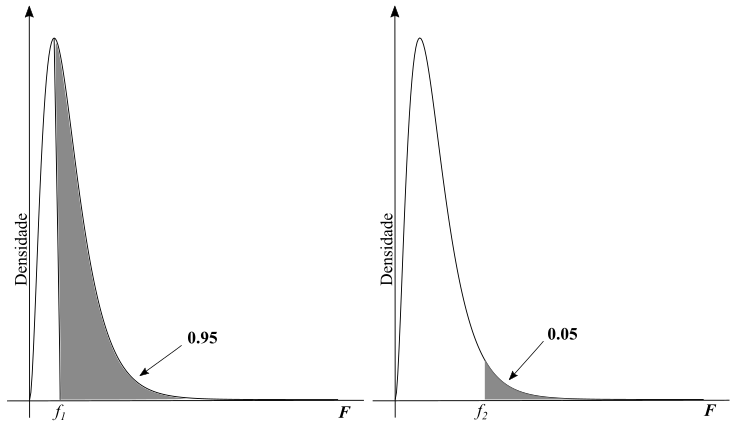
\includegraphics[width=0.9\linewidth]{figs/figura_92b} \end{center}
\end{frame}

\setbeamercovered{transparent}
\begin{frame}
\frametitle{Etapa 4: Calculando a estatística do teste (ANOVA independente)}
Você calcula o $SQ_{entre}$ calculando a SQ para as médias dos três grupos e depois multiplicando esse valor $SQ_{medias}$ por \textit{m} (o número de unidades amostrais em cada grupo).

\begin{center}
\begin{tabular}{ccc} 
 \hline
Tratamento & Média ($\bar{Y}_i$) & $\bar{Y}_i^2$\\
 \hline
TCC & 8 & 64 \\
TFD & 15.5 & 240.25 \\
TN  & 16.333 & 266.777 \\
 \hline
 & $\bar{Y}=13.6$ & $\sum_{i=1}^K\bar{Y}_i^2 = 571.027$\\
 \hline
\end{tabular}
\end{center}   
 
\[SQE = m \sum_{i=1}^K(\bar{Y}_i-\bar{Y})^2 = m(\sum_{i=1}^K\bar{Y}_i^2-K\bar{Y}^2)\]

\[SQE =  6 \times (571.027- 3\times 13.6^2) = \]

\end{frame}

\setbeamercovered{transparent}
\begin{frame}
\frametitle{Etapa 4: Calculando a estatística do teste (ANOVA independente)}
Você encontra o $SQD$ calculando a SQ para cada condição de tratamento separadamente e depois somando-os.

\[SQD = \sum_{i=1}^K\sum_{j=1}^m (Y_{ij}-\bar{Y}_i)^2 = \sum_{i=1}^K\sum_{j=1}^m Y_{ij}^2 -m\sum_{i=1}^K\bar{Y}^2\]

\[SQ_{TCC} = \sum_{j=1}^m (Y_{1j}-\bar{Y}_1)^2 = 108\]

\[SQ_{TFD} = \sum_{j=1}^m (Y_{2j}-\bar{Y}_2)^2 = 57.5\]

\[SQ_{TN} = \sum_{j=1}^m (Y_{3j}-\bar{Y}_3)^2 = 143.333\]

\[SQD = 108+57.5+143.333=308.83\]
\end{frame}

\setbeamercovered{transparent}
\begin{frame}
\frametitle{Etapa 4: Calculando a estatística do teste (ANOVA independente)}
Você encontra o $SQD$ calculando a SQ para cada condição de tratamento separadamente e depois somando-os.

\[SQ_{TCC} = \sum_{j=1}^m (Y_{1j}-\bar{Y}_1)^2 = 108\]

\[SQ_{TFD} = \sum_{j=1}^m (Y_{2j}-\bar{Y}_2)^2 = 57.5\]

\[SQ_{TN} = \sum_{j=1}^m (Y_{3j}-\bar{Y}_3)^2 = 143.333\]

\[SQD = 108+57.5+143.333=308.83\]
\end{frame}

\setbeamercovered{transparent}
\begin{frame}
\frametitle{Etapa 4: Calculando a estatística do teste (ANOVA independente)}
Agora você precisa da SQtotal, que representa a variabilidade total em todo o conjunto de dados. Você soma o variabilidade entre condições (isto é, SQE) e a variabilidade dentro das condições (isto é, SQD).

\begin{align*}
SQT &= \sum_{i=1}^K\sum_{j=1}^m (Y_{ij}-\bar{Y})^2 \\
    &= \sum_{i=1}^K\sum_{j=1}^m Y_{ij}^2 -mK\bar{Y}^2\\
    &= SQE + SQD = 252.78 + 308.83 = 561.61
\end{align*}

Seu objetivo final é calcular o F obtido, que é a razão entre QMentre e QMerro. Para calcular os QMs, você divide cada valor das SQ por seu próprio valor de gl.
\end{frame}

\setbeamercovered{transparent}
\begin{frame}
\frametitle{Etapa 4: Calculando a estatística do teste (ANOVA independente)}

Seu objetivo final é calcular o F obtido, que é a razão entre QMentre e QMerro. Para calcular os QMs, você divide cada valor das SQ por seu próprio valor de gl.

\[QME = \frac{SQE}{K-1}=\frac{252.58}{2} = 126.39\]

\[QMD = \frac{SQD}{N-K}=\frac{252.58}{15} = 20.59\]

Seu F obtido é calculado dividindo o QME pelo QMD:

\[F = \frac{QME}{QMD} = \frac{126.39}{20.59} = 6.138\]
 
\end{frame}


\setbeamercovered{transparent}
\begin{frame}
\frametitle{Etapa 4: Calculando a estatística do teste (ANOVA independente)}
A discussão sobre o comportamento dos erros e das somas de quadrados é resumida na \textbf{Tabela de Análise de Variância (ANOVA)}:

\begin{table}[h]
\centering
\begin{tabular}{ccccc}
\hline
Fonte de & Graus de & Soma de & Quadrado & F  \\
Variação & Liberdade & Quadrados & Médio &   \\
\hline
Entre & K-1 & SQE & QME & QME/QMD   \\
Dentro & N-K & SQD & QMD &   \\
\hline
Total & N-1 & SQT &  &   \\
\hline
\end{tabular}

\end{table}
\end{frame}

\setbeamercovered{transparent}
\begin{frame}
\frametitle{Etapa 4: Calculando a estatística do teste (ANOVA independente)}
A Tabela 11.4 é a tabela fonte da ANOVA para esta análise. Confirme que você entende como cada um os valores SQs, gls, QMs e F foram calculados.

\begin{table}[h]
\centering
\begin{tabular}{ccccc}
\hline
Fonte de & Graus de & Soma de & Quadrado & F  \\
Variação & Liberdade & Quadrados & Médio &   \\
\hline
Entre & 2 & 258.72 & 126.39 & 6.14   \\
Dentro & 15 & 308.83 & 20.59 &   \\
\hline
Total & 17 & 561.61 &  &   \\
\hline
\end{tabular}
\end{table}

Neste caso, o valor F obtido foi 6.14, que é superior ao valor F crítico de 3.68 (\(\alpha = 0.05\)). Portanto, você rejeita a hipótese nula e conclui que pelo menos uma média amostral é significativamente diferente de uma das outras.


\end{frame}

\setbeamercovered{transparent}
\begin{frame}
\frametitle{4e. Se necessário, calcule testes post hoc}
A hipótese nula para uma ANOVA é que todas as diferentes médias das condições são iguais. \\~\\

Rejeitar a hipótese nula não indica quais pares de médias são diferentes entre si. Assim, se você rejeitar a hipótese nula e houver três ou mais condições VI no estudo, será necessário realizar testes post hoc de pares para determinar qual par ou pares de médias são diferentes entre si. 

\end{frame}

\setbeamercovered{transparent}
\begin{frame}
\frametitle{\textit{teste de diferença honestamente significativa (HSD) de Tukey}}

O teste HSD revela quão diferentes devem ser quaisquer duas médias para serem consideradas "improváveis de resultar de erro de amostragem". A fórmula HSD é

\[HSD = q\sqrt{\frac{SQD}{m}}\]

O valor de \textit{q} (chamado de estatística de faixa estudentizada) muda, com base no número de condições de tratamento (ou seja, K), o gl para o termo de erro e o valor alfa. Com base nesses valores, a estatística \textit{q} é 3.67.

Assim, seu valor HSD é

\[HSD = q\sqrt{\frac{SQD}{n}}= 3.67\sqrt{\frac{20.59}{6}}=6.80\]

\end{frame}

\setbeamercovered{transparent}
\begin{frame}
\frametitle{\textit{teste de diferença honestamente significativa (HSD) de Tukey}}

Conforme indicado na tabela, diferenças significativas sugerem que a diferença não foi criada por erro amostral.

\begin{table}[h]
\centering
\begin{tabular}{ccc}
\hline
Comparação & Diferença entre médias & Siginificância\\
\hline
TCC vs TFD & $|8-15.5|=7.5$ & $>HSD$ - Significativo\\
TCC vs NT & $|8-16.33|=8.33$ & $>HSD$ - Significativo\\
NT vs PDT & $|15.5-16.33|=-0.83$ & $<HSD$ - Não Significativo\\
\hline
\end{tabular}
\end{table}

\end{frame}


\begin{frame}
\frametitle{Etapa 5: calcule o tamanho do efeito e descreva-o}
Quando você tem dois grupos, usa d como medida do tamanho do efeito. Você não pode usar d como medida do tamanho do efeito para uma ANOVA geral porque geralmente há mais de dois grupos, então você não pode calcular uma diferença média simples. O tamanho do efeito mais comum para ANOVAs é eta parcial quadrado  ($\eta_p^2$). Os cálculos são os seguintes:

\[\eta_p^2 = \frac{SQE}{SQE+SQD}=\frac{252.78}{252.78+308.83}=0.45\]

Para ANOVAs de um fator, você deve interpretar o eta parcial quadrado como a porcentagem da variabilidade VD que a VI "explica". Neste caso, o tipo de tratamento que os participantes recebem "explica" 45\% da variabilidade nos seus valores de depressão. O tamanho do efeito obtido de 0.45 é maior que 0.14 e, portanto, é um efeito grande.

\end{frame}

\setbeamercovered{transparent}
\begin{frame}
\frametitle{Etapa 6: resumir os resultados}

Ao relatar uma ANOVA, as médias, desvios padrão e tamanhos de efeito para as comparações aos pares são relatados em tabelas, portanto não precisam ser repetidos no texto. O que se segue é um exemplo de como a análise acima pode ser resumida.\\~\\

Uma ANOVA independente revelou diferenças significativas entre as três terapias para depressão, F(2, 15) = 6.14, $p < 0.05$, $\eta_p^2 = 0.45$, QME = 20.59. As médias e desvios padrão para cada tratamento estão na Tabela de ANOVA. Os testes \textit{post hoc} do HSD de Tukey revelaram que o grupo da TCC apresentou valores de depressão mais baixos do que o grupo TFD e o grupo sem tratamento. A terapia TFD não foi melhor do que não receber nenhum tratamento. Os testes post hoc do HSD e seus tamanhos de efeito foram apresentados anteriormente.

\end{frame}

\setbeamercovered{transparent}
\begin{frame}
\frametitle{Uma nota adicional sobre ANOVAS}
Se você fizer vários testes t, cada teste t terá 5\% de chance de produzir um erro Tipo I. Se você realizar vários testes t, a probabilidade exata de ter cometido pelo menos um erro Tipo I é dada pela seguinte fórmula de erro familiar (\textit{family-wise error rate} - FWER)\\~\\

$FWER = 1-(1-\alpha)^c$, onde c é o número de comparações\\~\\

Se você tiver apenas uma comparação, a taxa de erro Tipo I seria\\~\\

$FWER = 1 - (1-0.05)^1 = 0.05$ ou 5\%.\\~\\


\end{frame}

\setbeamercovered{transparent}
\begin{frame}
\frametitle{Uma nota adicional sobre ANOVAS}
No entanto, se você tiver três comparações no mesmo estudo, a probabilidade de ter cometido pelo menos um erro Tipo I é um pouco maior, 0,14 ou 14\%.\\~\\

$FWER = 1 - (1 - 0.05)^3 = 0.14$.\\~\\

Fazer uma única ANOVA em vez de vários testes t mantém a taxa de erro familiar em 0.05 para a ANOVA geral. Se forem necessários testes \textit{post hoc}, há uma variedade de testes para escolher, mas a ideia geral por trás da maioria deles é que eles evitam que a taxa de erro Tipo I aumente.

\end{frame}

\setbeamercovered{transparent}
\begin{frame}
\frametitle{Exemplo 9.16}
A gerência de um depósito que armazena cargas aéreas de pequeno porte está estudando o peso das cargas que chegam ao seu terminal no interior de São Paulo. Usualmente, o terminal recebe 4 tipos de cargas: doméstica (D), administrativa (A), equipamentos industriais (E) e outros tipos (O). Deseja-se verificar se, em média, existem diferenças entre os pesos dos 4 tipos de cargas. Ao longo de 1 mês, cargas foram colhidas aleatoriamente e seus pesos foram aferidos, fornecendo os dados (em kg):

\begin{table}[h]
\tiny
\centering
\begin{tabular}{cccc}
\hline
& Tipos de Carga & & \\
\hline
D & A & E & O \\
24.9 & 27.9 & 38.4 & 23.8 \\
20.4 & 28.1 & 38.6 & 25.3 \\
24.2 & 28.4 & 41.2 & 23.5 \\
22.3 & 25.3 & 43.9 & 27.6 \\
20.3 & 29.3 & 40.2 & 25.5 \\
24.0 & 28.5 & 40.2 & 23.9 \\
23.5 & 27.9 & 37.3 & 22.6 \\

\hline
\end{tabular}
\end{table}
\end{frame}


\setbeamercovered{transparent}
\begin{frame}
\frametitle{Referências bibliográficas}
\printbibliography
\end{frame}

\end{document}